% SZTE Alkalmazott matematikus MSc záróvizsgatételek
%
% Szerzők:		Judák Regina
%				reginajudak@gmail.com
%
%				Majernyik Noel
%				majnol@vipmail.hu
%
%				Mezőfi Dávid
%				david.mezofi93@gmail.com
%
%%%%%%%%%%%%%%%%%%%%%%%%%%%%%%%%%%%%%%%%%%%%%%%%%%%%%%%%%%%%%%%%%%%%%%%%%%%%%%%%%%%%%%%%%%%%%%%%%%%%
%
% Creative Commons licenc
%
% Ez az alkotás a Creative Commons Nevezd meg! - Ne add el! - Így add tovább! 4.0 Nemzetközi licenc
% alá tartozik. A licenc megtekintéséhez látogass el a
% http://creativecommons.org/licenses/by-nc-sa/4.0/ oldalra.
%
%%%%%%%%%%%%%%%%%%%%%%%%%%%%%%%%%%%%%%%%%%%%%%%%%%%%%%%%%%%%%%%%%%%%%%%%%%%%%%%%%%%%%%%%%%%%%%%%%%%%
%
% PREAMBULUM
%
%%%%%%%%%%%%%%%%%%%%%%%%%%%%%%%%%%%%%%%%%%%%%%%%%%%%%%%%%%%%%%%%%%%%%%%%%%%%%%%%%%%%%%%%%%%%%%%%%%%%
%
% DIV=15 opcióval nem lesznek nagy margók, `twoside` opció a kétoldalas szedéshez.
\documentclass[DIV=15,appendixprefix]{scrreprt}
%
% Színes hivatkozásokhoz kommenteld ki az alábbi sort!
% Élő hivatkozások, indexek, PDF-ben, színesekhez: `colorlinks=true`
\usepackage[unicode,pdfborder={0 0 0}]{hyperref}
%
%%%%%%%%%%%%%%%%%%%%%%%%%%%%%%%%%%%%%%%%%%%%%%%%%%%%%%%%%%%%%%%%%%%%%%%%%%%%%%%%%%%%%%%%%%%%%%%%%%%%
%
% Karakterkódolás és `babel` beállítása.
\usepackage[T1]{fontenc}
\usepackage[utf8]{inputenc}
% A `defaults=hu-min` opció biztosítja, hogy a tizedesvessző tizedesvessző legyen.
\def\magyarOptions{%
	defaults=hu-min}
\usepackage[magyar]{babel}
%
% A `description` környzetek "szépen" jelenjenek meg.
\def\descriptionlabel#1{\hskip\labelsep\normalfont\sffamily\bfseries #1.}
%%%%%%%%%%%%%%%%%%%%%%%%%%%%%%%%%%%%%%%%%%%%%%%%%%%%%%%%%%%%%%%%%%%%%%%%%%%%%%%%%%%%%%%%%%%%%%%%%%%%
%
% Tételszerű bekezdések.
\usepackage{amsthm}
\usepackage{amsmath, amssymb}
%
% Tétel és társai: félkövér + dőlt
\newtheorem*{tetel}{Tétel}
\newtheorem*{allit}{állítás}
\newtheorem*{kovet}{Következmény}
%
% Definíció és társai: félkövér + álló
\theoremstyle{definition}
\newtheorem*{defin}{Definíció}
\newtheorem*{feladat}{Feladat}
%
% Megjegyzés és társai: dőlt + álló
\theoremstyle{remark}
\newtheorem*{megj}{Megjegyzés}
\newtheorem*{utmut}{Útmutatás}
\newtheorem*{pelda}{Példa}
%
%%%%%%%%%%%%%%%%%%%%%%%%%%%%%%%%%%%%%%%%%%%%%%%%%%%%%%%%%%%%%%%%%%%%%%%%%%%%%%%%%%%%%%%%%%%%%%%%%%%%
%
% Számozások
%
% A feladat környzet számozása 17-tel kezdődik.
%\addtocounter{feladat}{16}
%
% Az egyenletek számozása szakaszokkal együtt történjen.
%\numberwithin{equation}{section}
%
%%%%%%%%%%%%%%%%%%%%%%%%%%%%%%%%%%%%%%%%%%%%%%%%%%%%%%%%%%%%%%%%%%%%%%%%%%%%%%%%%%%%%%%%%%%%%%%%%%%%
%
% Szépen szedett algoritmusok.
%
\usepackage[ruled,section]{algorithm}
\usepackage[noend]{algpseudocode}
\algrenewcommand\algorithmicrequire{\textbf{Bemenet}:}
\algrenewcommand\algorithmicensure{\textbf{Kimenet}:}
\newcommand{\Break}{\State\textbf{break} }
%
\usepackage{caption}
\makeatletter
\renewcommand{\ALG@name}{algoritmus}
\makeatother
\makeatletter
\DeclareCaptionLabelFormat{hunalg}{#2.~\ALG@name.}
\makeatother
\captionsetup[algorithm]{labelformat=hunalg}
% Példa.
%
%\begin{algorithm}
%	\caption{Cím}
%	\begin{algorithmic}
%		\Procedure{Kiír}{}
%			\While{$\diamond$ utáni bináris szám nem 0}
%				\State Kiírjuk a munkaszalag $\diamond$-ig lévő tartalmát, $a^{n}$-t.%
%					\Comment{Folytatólagosan írunk.}
%				\State Csökkentjük 1-gyel a $\diamond$ utáni bináris számot.%
%					\Comment{Vonjunk ki belőle 1-et.}
%			\EndWhile
%		\EndProcedure
%	\end{algorithmic}
%\end{algorithm}
%
%%%%%%%%%%%%%%%%%%%%%%%%%%%%%%%%%%%%%%%%%%%%%%%%%%%%%%%%%%%%%%%%%%%%%%%%%%%%%%%%%%%%%%%%%%%%%%%%%%%%
%
% Egyebek
%
% Grafikai csomagok betöltése.
\usepackage{graphicx}
%\usepackage{eso-pic}
%
% A képek elérési útvonalának megadása.
%\graphicspath{{./figures/}}
% Nyomdai minőségű táblázatok készítéséhez a `booktabs` csomag szükséges.
%\usepackage{booktabs}
%
% "Dummy" szöveg: Lipsum dolor sit amet...
\usepackage{lipsum}
%
% Szövegközi "ferdetört". Használat: `\sfrac{num}{den}`.
%\usepackage{xfrac}
%
% Az `enumitem` csomag színes-szagos `enumerate` környezetet biztosít.
\usepackage{enumitem}
\setlist[description]{labelindent=\parindent}
% Példa a használatra:
%
%\begin{enumerate}[label = (H-\arabic{*}), ref = H-\arabic{*}, leftmargin = *,%
%		 labelindent = \parindent, mode = unboxed]
%	\item
%\end{enumerate}
%
% Az írógép típusú betűtípus legyen Inconsolata.
% Másik hasznos a `courier`: ha dőlt, félkövér és egyebek is kellenek.
%\usepackage{inconsolata}
%
% Többsoros kommentek `verbatim` környezettel.
%\usepackage{verbatim}
%
% A következő csomag feltételezi, hogy van működő SAGE telepítve a SageTex csomaggal együtt.
%\usepackage{sagetex}
%
% Kontinentális mondatközök.
\frenchspacing
%
% Fejezetcímek magyar formátumnak megfelelően.
\renewcommand*{\chapterformat}{\thechapter\autodot\ \chapappifchapterprefix.\enskip}
%
% Minden szakasz új oldalon kezdődjön.
\usepackage{titlesec}
\newcommand{\sectionbreak}{\clearpage}
%
%%%%%%%%%%%%%%%%%%%%%%%%%%%%%%%%%%%%%%%%%%%%%%%%%%%%%%%%%%%%%%%%%%%%%%%%%%%%%%%%%%%%%%%%%%%%%%%%%%%%
%
% Saját matematikai parancsok:
\newcommand{\ball}{\mathbb{B}}
\newcommand{\sphere}{\mathbb{S}}
\newcommand{\mean}{\mathbb{E}}
\newcommand{\prob}{\mathbb{P}}
\newcommand{\sd}{\mathbb{D}}
\newcommand{\BinomialD}{\mathcal{B}}
\newcommand{\imag}{\mathfrak{i}}
\newcommand{\SAGE}{\textsf{\textbf{SAGE}}{}}
\renewcommand{\tan}{\mathop{\mathrm{tg}}}
\DeclareMathOperator{\conv}{conv}
\DeclareMathOperator{\interior}{int}
\newcommand{\ballin}{\interior\mathbb{B}}
\DeclareMathOperator{\relint}{relint}
\DeclareMathOperator{\cl}{cl}
\DeclareMathOperator{\T}{T}
\DeclareMathOperator{\supp}{supp}
\DeclareMathOperator{\dom}{dom}
\DeclareMathOperator{\diag}{diag}

%
%%%%%%%%%%%%%%%%%%%%%%%%%%%%%%%%%%%%%%%%%%%%%%%%%%%%%%%%%%%%%%%%%%%%%%%%%%%%%%%%%%%%%%%%%%%%%%%%%%%%
%
% Cím és társai
%
\titlehead{Szegedi Tudományegyetem\\%
	Természettudományi és Informatikai Kar\\%
	Bolyai Intézet}
\subject{Alkalmazott matematikus MSc}
\title{Záróvizsgatételek}
\subtitle{Általános szakirány}
\author{Judák Regina\\\texttt{reginajudak@gmail.com}%
	\and%
	Majernyik Noel\\\texttt{majnol@vipmail.hu}
	\and%
	Mezőfi Dávid\\\texttt{david.mezofi93@gmail.com}}
\date{Utoljára módosítva: \today}
%\publishers{asd}
%%%%%%%%%%%%%%%%%%%%%%%%%%%%%%%%%%%%%%%%%%%%%%%%%%%%%%%%%%%%%%%%%%%%%%%%%%%%%%%%%%%%%%%%%%%%%%%%%%%%
%
% DOKUMENTUM
%
%%%%%%%%%%%%%%%%%%%%%%%%%%%%%%%%%%%%%%%%%%%%%%%%%%%%%%%%%%%%%%%%%%%%%%%%%%%%%%%%%%%%%%%%%%%%%%%%%%%%
%
\begin{document}
%
% Cím
\maketitle
%
% Licenc
\minisec{Creative Commons licenc}
\begin{center}
	\includegraphics{by-nc-sa.eps}
\end{center}
Ez az alkotás a \emph{Creative Commons Nevezd meg! -- Ne add el! -- Így add tovább! 4.0 Nemzetközi
licenc} alá tartozik. A licenc megtekintéséhez látogass el a
\url{http://creativecommons.org/licenses/by-nc-sa/4.0/} oldalra.
%
% Tartalomjegyzék
\tableofcontents
%
%%%%%%%%%%%%%%%%%%%%%%%%%%%%%%%%%%%%%%%%%%%%%%%%%%%%%%%%%%%%%%%%%%%%%%%%%%%%%%%%%%%%%%%%%%%%%%%%%%%%
%
% Mindkét szakirányon közös tételek
%
\chapter{Mindkét szakirányon közös tételek}
%
\section{Gráfelmélet: összefüggőség, színezések}
%
\section{Gráfelmélet: párosítások, síkgráfok}
%
\section{Gröbner-bázisok és alkalmazásaik}
%
\section{Matematikai titkosírások}
%
\section{Többváltozós és vektorértékű függvények}
%
\section{Fourier-sorok, ortogonális polinomok, sorfejtések}
%
\section{Közönséges differenciálegyenletek és elsőrendű parciális differenciálegyenletek}
%
\section{Többdimenziós normális eloszlású vektorok statisztikai analízise}
%
\section{Lineáris regresszió}
%
\section{Kontingenciatáblák elemzése}
%
\section{Diszkrét idejű Markov-láncok}
%
\section{Folytonos idejű Markov-láncok}
%
\section{Sztochasztikus folyamatok alapfogalmai}
%
\section{Optimalizálási eljárások}
%
\minisec{Alapfeladat és speciális esetei}
Legyen $ c \colon \mathbb{ R }^{ n } \supseteq \dom c \rightarrow \mathbb{ R } $ a
\emph{célfüggvény}, ekkor az optimalizálás feladata a $ c $ célfüggvény minimalizálása előre
kiszabott feltételek mellett:
\begin{equation*}
	\begin{array}{rcl}
		\mathbf{ x }					&	\in			&	\mathcal{ F }\\
		\hline
		c \left( \mathbf{ x } \right)	&	\rightarrow	&	\min
	\end{array} \quad \left( \mathbf{ x } \in \dom c \right).
\end{equation*}
Explicit feltételek:
\begin{equation*}
	\begin{cases}
		f_{ i } \left( \mathbf{ x } \right) \le 0,	&	i \in \left[ k \right] = \left\{ 1,{} 2,{}
			\ldots,{} k \right\};\\
		g_{ j } \left( \mathbf{ x } \right) = 0,	&	j \in \left[ \ell \right],
	\end{cases} \quad \Rightarrow \quad \begin{cases}
		f \left( \mathbf{ x } \right) \preceq \mathbf{ 0 };	&\\
		g \left( \mathbf{ x } \right) = \mathbf{ 0 }.		&
	\end{cases}
\end{equation*}
A $ \mathcal{ D } $ \emph{értelmezési tartomány} a $ c $, az $ f_{ i } $ és a $ g_{ j } $ függvények
értelmezési tartományainak metszete. A \emph{lehetséges megoldások halmaza}: $ \mathcal{ L } =
\mathcal{ D } \cap \mathcal{ F } $. Az $ \left( \mathbf{ x }^{ * },{} p^{ * } \right) $ párt
\emph{optimális helynek}, illetve \emph{optimális értéknek} nevezzük, ha
\begin{equation*}
	c \left( \mathbf{ x }^{ * } \right) = p^{ * } = \inf_{ \mathbf{ x } \in \mathcal{ L } } c \left(
	\mathbf{ x } \right) \in \mathbb{ R } \cup \left\{ - \infty \right\} \cup \left\{ \infty
	\right\}.
\end{equation*}
Gyakran megelégszünk \emph{$ \epsilon $-közelítő} $ \left( p^{ * } + \epsilon \right) $, illetve
\emph{-approximáló} $ \left( \left( 1 + \epsilon \right) p^{ * },{} \left( 1 - \epsilon \right)
p^{ * } \right) $ megoldásokkal. A problémák átfogalmazhatók a feltételek ekvivalens átalakításával,
\emph{slack}-változók bevezetésével (egyenlőtlenség kiküszöbölésére), valamint a célfüggvény monoton
függvénybe történő helyettesítésével.
\begin{description}
	\item[Feltétel nélküli optimalizálás] Legkisebb négyzetek problémája: $ \left\| \mathbf{ c } -
		\mathbf{ A } \mathbf{ x } \right\|^{ 2 } \rightarrow \min $ (egyenes illesztése mért
		adatpontokra)
	\item[LP-feladatok] \begin{equation}\tag{LP}
			\begin{array}{rcl}
				\mathbf{ A } \mathbf{ x }			&	=			&	\mathbf{ b }\\
				\mathbf{ x }						&	\succeq		&	\mathbf{ 0 }\\
				\hline
				\mathbf{ c }^{ \T } \mathbf{ x }	&	\rightarrow	&	\min
			\end{array}, \qquad \begin{array}{rcl}
				\mathbf{ A } \mathbf{ x }			&	\preceq		&	\mathbf{ b }\\
				\hline
				\mathbf{ c }^{ \T } \mathbf{ x }	&	\rightarrow	&	\min
			\end{array}.
		\end{equation}
	\item[SDP-feladatok] \begin{equation}\tag{SDP}
			\begin{array}{rcl}
				\sum_{ i = 1 }^{ n } x_{ i } \mathbf{ A }_{ i }		&	\preceq	&	\mathbf{ B }\\
				\mathbf{ D } \mathbf{ x }							&	=	&	\mathbf{ e }\\
				\hline
				\mathbf{ c }^{ \T } \mathbf{ x }	&	\rightarrow	&	\min
			\end{array}; \qquad \underbrace{\begin{array}{rcll}
				\left\langle \mathbf{ A }_{ i },{} \mathbf{ X } \right\rangle	&	=	&
					b_{ i }			&	i \in \left[ k \right]\\
				\mathbf{ X }													&	\succeq	&
					\mathbf{ 0 }	&\\
				\hline
				\left\langle \mathbf{ C },{} \mathbf{ X } \right\rangle			&	\rightarrow	&
					\min			&
			\end{array}}_{\text{I. normálforma}}; \qquad \underbrace{\begin{array}{rcl}
				\sum_{ i = 1 }^{ n } x_{ i } \mathbf{ A }_{ i }		&	\preceq	&	\mathbf{ B }\\
				\hline
				\mathbf{ c }^{ \T } \mathbf{ x }	&	\rightarrow	&	\min
			\end{array}}_{\text{II. normálforma}},
		\end{equation}
		ahol az $ \mathbf{ A }_{ i },{} \mathbf{ B },{} \mathbf{ C },{} \mathbf{ X } $ mátrixok
		szimmetrikusak.
\end{description}
%
\minisec{Lagrange-módszer}
\begin{equation*}\tag{Lagrange-függvény}
	L \left( \mathbf{ x };{} \lambda,{} \mu \right) = c \left( \mathbf{ x } \right) + \lambda^{ \T }
	f \left( \mathbf{ x }	\right) + \mu^{ \T } g \left( \mathbf{ x }	\right).
\end{equation*}
Ha $ \mathbf{ x } \in \mathcal{ L } $ és $ \lambda \succeq \mathbf{ 0 } $, akkor $ c \left(
\mathbf{ x } \right) \ge L \left( \mathbf{ x };{} \lambda,{} \mu \right) $. Így
\begin{equation}\tag{duális célfüggény, duális feladat}
	\tilde{ c } \left( \lambda,{} \mu \right) = \inf_{ \mathbf{ x } \in \mathcal{ D } } L \left(
	\mathbf{ x };{} \lambda,{} \mu \right), \qquad \begin{array}{rcl}
		\lambda										&		\succeq	&	\mathbf{ 0 }\\
		\hline
		\tilde{ c } \left( \lambda,{} \mu \right)	&	\rightarrow	&	\max
	\end{array}.
\end{equation}
\begin{tetel}[gyengedualitás-tétel]
	Legyen a duális feladat optimális értéke $ d^{ * } $. Ekkor $ p^{ * } \ge d^{ * } $.
\end{tetel}
\begin{megj}
	Ha egyenlőség teljesül, akkor \emph{erős dualitás}. Ha $ p^{ * } - d^{ * } > 0 $, akkor
	\emph{pozitív dualitási hézag}.
\end{megj}
%
\minisec{Karush\,--\,Kuhn\,--\,Tucker-tétel}
Tegyük fel, hogy $ g_{ i } $-k affin, $ c,{} f_{ i } $-k konvex és differenciálható függvények. Erős dualitás pontosan akkor teljesül, ha létezik $ \hat{ \mathbf{ x } } $, $ \left( \hat{ \lambda }
,{} \hat{ \mu } \right) $, melyek teljesítik a következő feltételeket:
\begin{enumerate}[label = (KKT--\arabic{*}), ref = KKT--\arabic{*}, mode = unboxed,%
	labelindent = \parindent, leftmargin = *]
	\item\label{kkt1} $ \hat{ \mathbf{ x } } $ primál lehetséges megoldás;
	\item\label{kkt2} $ \left( \hat{ \lambda },{} \hat{ \mu } \right) $ duál lehetséges megoldás;
	\item\label{kkt3} $ \hat{ \mathbf{ x } } $, $ \left( \hat{ \lambda },{} \hat{ \mu } \right) $
	komplementárisan laza tulajdonságú, azaz
		\begin{itemize}
			\item ha $ f_{ i } \left( \hat{ \mathbf{ x } } \right) < 0 $, akkor
				$ \hat{ \lambda }_{ i } = 0 $;
			\item ha $ \hat{ \lambda }_{ i } > 0 $, akkor $ f_{ i } \left( \hat{ \mathbf{ x } }
				\right) = 0 $;
		\end{itemize}
	\item\label{kkt4} $ \nabla c \left( \hat{ \mathbf{ x } } \right) + \left( \hat{ \lambda }
		\right)^{ \T } \nabla f \left( \hat{ \mathbf{ x } } \right) + \left( \hat{ \mu }
		\right)^{ \T } \nabla g \left( \hat{ \mathbf{ x } } \right) = 0 $.
\end{enumerate}
Ha létezik ilyen $ \hat{ \mathbf{ x } } $, $ \left( \hat{ \lambda } ,{} \hat{ \mu } \right) $, akkor $ \hat{ \mathbf{ x } } $ primál, $ \left( \hat{ \lambda } ,{} \hat{ \mu } \right) $ duál optimumhely.
%
\minisec{Súlyozott párosítási probléma}
\begin{feladat}
	Legyen a $ G $ gráf, valamint a $ c \colon E \rightarrow \mathbb{ R }^{ + } $ \emph{élsúlyozás}
	adott. Keressünk maximális súlyú párosítást!
\end{feladat}
A $ c $ súlyfüggvényt azonosíthatjuk egy $ \mathbf{ c } \in \mathbb{ R }^{ E } $ vektorral. Legyen
$ \mathbf{ B } $ a $ G $ gráf \emph{pont-él illeszkedési mátrixa}. Így a feladat:
\begin{equation*}
	\underbrace{\begin{array}{rcl}
		\mathbf{ B } \mathbf{ x }			&	\preceq	&	\mathbf{ 1 }\\
		\mathbf{ 0 }						&	\preceq	&	\mathbf{ x }\\
		\mathbf{ x }						&	\in		&	\mathbb{ Z }^{ E }\\
		\hline
		\mathbf{ c }^{ \T } \mathbf{ x }	&	\rightarrow	&	\max
	\end{array}}_{\text{egész feltételű LP}} \qquad \leadsto \qquad \underbrace{\begin{array}{rcl}
		\mathbf{ B } \mathbf{ x }			&	\preceq	&	\mathbf{ 1 }\\
		\mathbf{ 0 }						&	\preceq	&	\mathbf{ x }\\
		\hline
		\mathbf{ c }^{ \T } \mathbf{ x }	&	\rightarrow	&	\max
	\end{array}}_{\text{LP-relaxáció}} \qquad \Leftrightarrow \qquad \begin{array}{rcl}
		\mathbf{ M } \mathbf{ x }			&	\preceq	&	\begin{bmatrix}
				\mathbf{ 1 }\\
				\mathbf{ 0 }
			\end{bmatrix}\\
		\hline
		\mathbf{ c }^{ \T } \mathbf{ x }	&	\rightarrow	&	\max
	\end{array} \quad \left( \mathbf{ M } = \begin{bmatrix}
		\mathbf{ B }\\
		- \mathbf{ I }_{ E }
	\end{bmatrix} \right) .
\end{equation*}
Ha $ G $ \emph{páros}, akkor $ \mathbf{ B } $ (és így $ \mathbf{ M } $ is) \emph{totálisan
unimoduláris} (bármely aldeterminánsa $ - 1 $, $ 0 $ vagy $ 1 $), és ekkor a relaxált feladat
ekvivalens az eredetivel.
%
\minisec{LP és SDP kombinatorikai alkalmazásai}\leavevmode
\begin{description}
	\item[Folyamprobléma és duálisa] Legyen $ \mathcal{ H } = \left( \vec{ G },{} s,{} t,{} c
		\right) $ hálózat: $ s,{} t $ rendre \emph{forrás}, \emph{nyelő}, $ c $
		\emph{kapacitásfüggény} $ \left( \mathbf{ c } \right) $. Legyen a \emph{folyamfüggvény} $ f
		\colon E \rightarrow \mathbb{ R } $, azonosíthatjuk $ \mathbf{ x } $-szel.
		Teljesüljenek a kapacitásfeltételek: $ \mathbf{ 0 } \preceq \mathbf{ x } \preceq
		\mathbf{ c } $, valamint a Kirchhoff-törvény (csúcsonként a ki- és a beáramló mennyiség
		azonos). A folyam \emph{értéke}: $ v $, a forrásnál a kiáramló és beáramló mennyiség
		különbsége (nyelőnél fordítva).

		Adjunk hozzá $ \vec{ G } $-hez egy $ e_{ + } = \overrightarrow{ t s } $ élt, melyen a
		(kiterjesztett) folyam $ v $-t vesz fel. Ekkor $ \vec{ G }_{ + } $ cirkuláció.  A feladat és
		duálisa:
		\begin{equation}\tag{MFMC}
			\begin{array}{rclcl}
				\mathbf{ 0 }							&	\preceq		&	\mathbf{ x }	&	\preceq	&	\mathbf{ c }\\
				\mathbf{ B }_{ + } \mathbf{ x }_{ + }	&	=			&	\mathbf{ 0 }	&			&	\\
				\hline
				v										&	\rightarrow	&	\max
			\end{array} \qquad \leadsto\qquad \begin{array}{rcl}
				\mathcal{ V }					&				& \text{egy $ s $-$ t $-vágás}\\
				\hline
				C \left( \mathcal{ V } \right)	&	\rightarrow	&	\min
			\end{array}.
		\end{equation}
	\item[Maximális vágás problémája és duálisa] Legyen $ G = \left( V,{} E \right) $ egyszerű gráf.
		Keressünk olyan $ \mathcal{ V } $ vágást, melyre $ \left| E \left( \mathcal{ V } \right)
		\right| $ maximális! A feladat duálisa SDP-feladat ($ \mathbf{ A } $ a szomszédsági mátrix,
		$ \mathbf{ x } \in \left\{ -1,{} 1 \right\}^{ V } $ a vágást kódolja):
		\begin{equation*}
			\begin{array}{rcl}
				\mathbf{ A } + \diag \mu 	&		\succeq	&	\mathbf{ 0 }\\
				\hline
				- \mathbf{ 1 }^{ \T } \mu	&	\rightarrow	&	\max
			\end{array}.
		\end{equation*}
%		Egy $ \mathcal{ V } $ vágás: $ \mathbf{ x } \in \left\{ -1,{} 1 \right\}^{ V } \subset
%		\mathbb{ R }^{ V } $, ahol a komponens $ - 1 $, ha a megfelelő csúcs a vágás egyik, $ 1 $,
%		ha a vágás másik oldalára esik. Legyen $ \mathbf{ A } $ a gráf szomszédsági mátrixa. Az
%		$ \mathbf{ x }^{ \T } \mathbf{ A } \mathbf{ x } $ kvadratikus alakban az $ e = \left\{ u,{}
%		v \right\} $ él hozzájárulása $ 2 x_{ u } x_{ v } $, $ x_{ u } x_{ v } = 1 $, ha $ e $-t
%		\textqq{nem vágtuk ketté}, $ - 1 $ különben. A feladat és duálisa:
%		\begin{equation*}
%	 		\begin{array}{rcl}
%				x_{ v }^{ 2 } 									&		=		& 1 \quad \left(
%				\forall \, v \in V \right)\\
%				\hline
%				\mathbf{ x }^{ \T } \mathbf{ A } \mathbf{ x }	&	\rightarrow	&	\min
%			\end{array} \qquad \leadsto \qquad \begin{array}{rcl}
%				\mathbf{ A } + \diag \mu 	&		\succeq	&	\mathbf{ 0 }\\
%				\hline
%				- \mathbf{ 1 }^{ \T } \mu	&	\rightarrow	&	\max
%			\end{array}.
%		\end{equation*}
	\item[Maximális független ponthalmaz felső becslése]  Legyen $ G = \left( V,{} E \right) $
		egyszerű gráf, legyen $ \mathbf{ A } $ a gráf szomszédsági mátrixa. Jelölje $ \mathbf{ J } $
		a csupa 1 mátrixot, legyen $ \bar{ \mathbf{ A } } = \mathbf{ J } - \mathbf{ A } $. Ekkor, ha
		$ F \subseteq V $ független ponthalmaz, akkor $ \left. \bar{ \mathbf{ A } }
		\right|_{ F \times F } = \mathbf{ J } $. Sajátvektor-sajátértékekre vonatkozó
		észrevételekből adódik, hogy $ \left| F \right| \le \lambda_{ \max } \left(
		\bar{ \mathbf{ A } } \right) $, és így $ \alpha \left( G \right)  \le \lambda_{ \max }
		\left( \bar{ \mathbf{ A } } \right) $.

		A kapcsolódó SDP-feladat:
%
%		Nevezzünk egy $ V \times V $-s szimmetrikus $ \mathbf{ M } $ mátrixot \emph{$ T_{ G }
%		$-tulajdonságúnak}, ha a főátlón és a \textqq{neméleknél} is 1-es szerepel. Ekkor az ilyen
%		tulajdonságú mátrixok maximális sajátérékeinek minimuma is alkalmas felső becslés $ \alpha
%		\left( G \right) $-re. Így, ha $ \mathbf{ S }_{ e } $ az $ e $ élnek megfelelő szomszédsági
%		mátrix, akkor az SDP-feladat:
		\begin{equation*}
	 		\begin{array}{rcl}
				\mathbf{ M } 									&		=		& \mathbf{ J } -
					\sum_{ e \in E } x_{ e } \mathbf{ S }_{ e }\\
				\mu \mathbf{ I }_{ V } - \mathbf{ M }			&		\succeq	& \mathbf{ 0 }\\
				\hline
				\mu	&	\rightarrow	&	\min.
			\end{array}
		\end{equation*}
		Ennek a feladatnak a optimumát a \emph{$ G $ gráf Lovász-féle $ \theta $-függvényének}
		nevezzük, és $ \alpha \left( G \right) \le \theta \left( G \right) $.

		\emph{Lovász-féle szendvicstétel}: $ \alpha \left( G \right) \le \theta \left( G \right) \le
		\bar{ \chi } \left( G \right) \left( = \chi \left( \bar{ G } \right) \right) $.
\end{description}
%
\minisec{Egészértékű programozás}
\begin{equation}\tag{IP és LP-relaxáltja}
	\begin{array}{rcl}
		\mathbf{ A } \mathbf{ x } 			&	\preceq		&	\mathbf{ b }\\
		\mathbf{ x } 						&	\in			&	\mathbb{ N }^{ n }\\
		\hline
		\mathbf{ c }^{ \T } \mathbf{ x }	&	\rightarrow	&	\min.
	\end{array} \qquad \leadsto \qquad \begin{array}{rcl}
		\mathbf{ A } \mathbf{ x } 			&	\preceq		&	\mathbf{ b }\\
		\hline
		\mathbf{ c }^{ \T } \mathbf{ x }	&	\rightarrow	&	\min.
	\end{array}
\end{equation}
\begin{description}
	\item[L-következtetés] Szokásos \textqq{levezetés} révén nyert új egyenlőtlenség.
	\item[I-következtetés] Ha $ \alpha_{ 1 } x_{ 1 } + \alpha_{ 2 } x_{ 2 } + \ldots +
		\alpha_{ n } x_{ n } \le \beta $ Az egyenlőtlenségek egy következménye
		(L-következtetés), akkor $ \left\lfloor \alpha_{ 1 } \right\rfloor x_{ 1 } +
		\left\lfloor \alpha_{ 2 } \right\rfloor x_{ 2 } + \ldots + \left\lfloor \alpha_{ n }
		\right\rfloor x_{ n } \le \left\lfloor \beta \right\rfloor $ egy \emph{I-köveztetés}. Az
		új egyenlőtlenségnek a feltételekhez történő hozzáadásával nem veszítünk lehetséges
		megoldást.
	\item[Algoritmus] L- és I-következtetések végrehajtását (valamilyen sámát követve, pl.
		Gomory-al\-go\-rit\-must) követően megoldjuk a kapcsolódó LP-relaxált feladatot, ha a kapott
		megoldás egész koordinátájú, akkor készen vagyunk, ha nem, akkor új L- és
		I-következtetéseket hajtunk végre, és így tovább\ldots
%		\leavevmode%
%		\begin{algorithmic}[1]
%			\Procedure{Relaxáció}{IP-feladat}
%				\State Oldjuk meg az IP-feladat LP-relaxáltját!
%				\State\Return az LP-relaxált feladat optimumhelye
%			\EndProcedure
%			\Procedure{GoodLuck}{optimumhely}
%				\If{optimumhely egész koordinátájú}
%					\State\Return \textsc{true}
%					\Else
%						\State\Return \textsc{false}
%				\EndIf
%			\EndProcedure
%			\Procedure{MegoldIP}{IP-feladat}
%				\State optimumhely $\gets$ \Call{Relaxáció}{IP-feladat}
%				\If{\Call{GoodLuck}{optimumhely}}
%					\State\Return optimumhely
%					\Else
%					\State új IP-feladat $\gets$ L- és I-következtetések\Comment{Gomory-algoritmus}
%					\State\Call{MegoldIP}{új IP-feladat}
%				\EndIf
%			\EndProcedure
%		\end{algorithmic}
\end{description}
%
\minisec{Korlátozás és szétválasztás módszerek alkalmazásai}
\begin{description}
	\item[Feltétel nélküli optimalizálás] $ c \left( \mathbf{ x } \right) $-et szeretnénk
		minimalizálni (létezik optimum, elég egy $ \epsilon $-kö\-ze\-lí\-tő megoldás). Legyen adott egy
		$ T_{ 0 } $ tégla, aminek eleme az optimumhely. Tegyük fel, hogy $ c $ \textqq{szép}: minden
		téglán könnyen adhatunk alső és felső becslést $ c $-re; egy téglalap (egy oldala menti)
		kettévágásával ezek a becslések javulnak; ha a téglalap egy ponthoz közelít, akkor az alsó
		és felső becslések különbsége kicsi $ \left( \epsilon \right) $ lesz.

		Az algoritmus dióhéjban: Téglalapfelezgetéssel közelítünk egy $ \epsilon $-közelítő
		megoldáshoz; egy téglát a leghosszabb oldala mentén felezünk; azon tégla \textqq{irányába}
		indulunk, amelyikre a legkisebb az alsó becslés (csak a \textqq{leveleket} tartjuk számon).
	\item[Vegyes konvex-egész optimalizálás] Legyen $ \mathbf{ d } \in \left\{ 0,{} 1
		\right\}^{ m } $, $ c $, $ f_{ i } $ $ \left( i \in \left[ k \right] \right) $ konvex függvények. A feladat:
		\begin{equation*}
			\begin{array}{rcl}
				f \left( \mathbf{ x },{} \mathbf{ d } \right) 	&	\preceq			& 0\\
				\hline
				c \left( \mathbf{ x },{} \mathbf{ d } \right) 	&	\rightarrow	&	\min
			\end{array}.
		\end{equation*}
	\item[Kevés nemnulla komponens lineáris feltételek mellett] Egy egyenlőtlenségrendszer olyan,
	megoldását keressük, melynek kevés nem nulla komponense van. Ez visszavezethető egy vegyes
	konvex-egész optimalizálási feladatra.
\end{description}
%
%%%%%%%%%%%%%%%%%%%%%%%%%%%%%%%%%%%%%%%%%%%%%%%%%%%%%%%%%%%%%%%%%%%%%%%%%%%%%%%%%%%%%%%%%%%%%%%%%%%%
%
% Általános szakirány tételei
%
\chapter{Általános szakirány tételei}
%
\section{Mátrixok sajátértékeinek meghatározása}
%
A tételhez kapcsolódó anyagrészek megtalálhatóak
\begin{enumerate}[label = (MF--\arabic{*}), ref = MF--\arabic{*}, mode = unboxed,%
	labelindent = \parindent, leftmargin = *]
	\item\label{mf1} \textsc{Móricz Ferenc}: \emph{Bevezetés a numerikus matematikába};
	\item\label{mf2} \textsc{Móricz Ferenc}: \emph{Numerikus módszerek az algebrában és analízisben}
\end{enumerate}
című könyveiben.
\minisec{Mátrixok trianguláris felbontása, ortogonális triangularizáció}
Lásd \ref{mf2} I. fejezet, 1. szakasz.

Egy $ \mathbf{ A } $ négyzetes mátrix \emph{trianguláris felbontása} ($ \mathbf{ A } = \mathbf{ L }
\mathbf{ U } $) nem minden esetben létezik, még akkor sem, ha a mátrix nemszinguláris. Viszont ha a
balfelső főminorok mind 0-tól különbözőek, akkor a felbontás létezik és a felső trianguláris
$ \mathbf{ U } $ mátrix diagonális elemei a balfelső főminorok segítségével meghatározhatóak és
ekkor $ \mathbf{ U } $ sem szinguláris. Ha az $ \mathbf{ A } $ mátrix valamely balfelső főminora
abszolútértékben kicsi, akkor a trianguláris felbontás során fellépő osztások során olyan kerekítési
hibák léphetnek fel, amelyek az eljárás végehajthatóságát veszélyeztethetik a túl kicsi/nagy
számokkal történő számolások következtében, vagy pedig teljesen eltorzíthatják az $ \mathbf{ L } $
és $ \mathbf{ U } $ mátrixok elemeit. Ez a probléma kiküszöbölhető egy másik típusú, ún.
\emph{ortogonális triangularizáció} segítségével, ahol az alulról trianguláris $ \mathbf{ L } $
mátrixot egy ortogonális $ \mathbf{ Q } $ mátrixszal helyettesítjük és egy felülről trianguláris
$ \mathbf{ U } $ mátrixot továbbra is megtartunk.

Ha az $ \mathbf{ A } $ mátrix nemszinguláris, akkor az $ \mathbf{ L } \mathbf{ U } $ felbontás
egyértelmű, míg a $ \mathbf{ Q } \mathbf{ U } $ felbontás a $ \mathbf{ Q } $ oszlopainak és
$ \mathbf{ U } $ sorainak előjelétől eltekintve egyértelmű.

Tetszőleges téglalap alakú mátrix ortogonális triangularizációja is definiálható a 3. tétel
segítségével.
%
\minisec{LR-algoritmus}
Lásd \ref{mf2} I. fejezet, 3. szakasz.

Legyen $ \mathbf{ A } $ négyzetes mátrix, melynek sajátértékeit meg szeretnénk határozni. Az
LR-algoritmus segítségével a következő módon határozhatjuk meg a sajátértékeket:
\begin{algorithmic}[1]
	\State $ \mathbf{ A }_{ 1 } \gets \mathbf{ A }$
	\State $ \left( \mathbf{ L }_{ 1 },{} \mathbf{ R }_{ 1 } \right) \gets $
		\Call{TriangulárisFelbontás}{$ \mathbf{ A }_{ 1 } $}
	\For{$ s \gets 1,{} s \gets s + 1$}
		\State $ \mathbf{ A }_{ s + 1 } \gets \mathbf{ R }_{ s } \mathbf{ L }_{ s } $
		\State $ \left( \mathbf{ L }_{ s + 1 },{} \mathbf{ R }_{ s + 1 } \right) \gets $ \Call{TriangulárisFelbontás}{$ \mathbf{ A }_{ s + 1 } $}
	\EndFor
\end{algorithmic}

Legyen $ \mathbf{ X } = \left[ \mathbf{ x }_{ 1 },{} \mathbf{ x }_{ 2 }, \ldots,{}
\mathbf{ x }_{ n } \right] $ az $ \mathbf{ A } $ sajátvektoraiból alkotott mátrix és $ \Lambda =
\diag \left[ \lambda_{ 1 },{} \lambda_{ 2 },{} \ldots,{} \lambda_{ n } \right]^{ \T } $ az
$ \mathbf{ A } $ sajátértékeiből képzett diagonális mátrix (feltéve, hogy $ \left| \lambda_{ 1 }
\right| > \left| \lambda_{ 2 } \right| > \ldots > \left| \lambda_{ n } \right| > 0 $). Ha
$ \mathbf{ X } $ és $ \mathbf{ X }^{ - 1 } $ balfelső főminorai 0-tól különbözőek, akkor az
$ \left\{ \mathbf{ A }_{ s } \colon s = 1,{} 2,{} 3,{} \ldots \right\} $ mátrixsorozat konvergens,
határértéke egy olyan felülről trianguláris mátrix, melynek főátlójában a $ \lambda_{ 1 },{}
\lambda_{ 2 },{} \ldots,{} \lambda_{ n } $ sajátértékek állnak.

Az előző algoritmus bármely lépésben elakadhat, ha nem létezik a trianguláris felbontás. Ha a
trianguláris felbontás során \emph{részleges főelemkiválasztást} alkalmazunk, akkor a
\emph{módosított LR-algoritmus} nem akadhat el, ha a szóban forgó mátrix nemszinguláris.
%
\minisec{QR-algoritmus}
Lásd \ref{mf2} I. fejezet, 4. szakasz.

Teljesen hasonló az LR-algoritmushoz, csak a trianguláris felbontás helyett ortogonális
triangularizációra van szükség.
%
\minisec{RHR-algoritmus}
Lásd \ref{mf1} II. fejezet, 5. szakasz.

\texttt{Ezt még nem néztem meg a másik Móricz-könyvben -- Regina.}
%
\section{Mátrixok általánosított inverze}
A tételhez kapcsolódó anyagrészek megtalálhatóak \ref{mf2} II. fejezetében.
%
\minisec{Motiváció}
Az \emph{általánosított inverz} bevezetésével definiálni tudunk egy olyan mátrixot szinguláris
négyzetes mátrixok és nem négyzetes mátrixok esetén is, amely hasonló tulajdonságokkal rendelkezik,
mint a hagyományos inverzmátrix, illetve négyzetes nemszinguláris mátrixok esetén megegyezik a
hagyományos inverzmátrixszal.
%
\minisec{Kiszámítás rangfaktorizációval}
Lásd \ref{mf1} II. fejezet, 6. szakasz.

Egy tetszőleges mátrix előállítható egy \emph{oszlopreguláris} és egy \emph{sorreguláris} mátrix
szorzataként (rangfaktorizáció). A sor-/oszlopreguláris mátrixok általánosított inverze számolható
az 1. és 2. definíciók szerint. Az általános definíciót ezen definíciók és a rangfaktorizáció
segítségével kapjuk.
%
\minisec{Kiszámítás particionálással}
Lásd \ref{mf1} II. fejezet, 8. szakasz.

Inverzmátrix \textsc{Forbenius} módszerével történő kiszámításának általánosítása. \emph{Rang
szerint particionált mátrix} általánosított inverze \textqq{könnyen} számítható a 29. tétel
segítségével. Tetszőleges mátrix két \emph{szimmetrikus permutáló mátrix} segítségével rang szerint
particionált alakra hozható, mely mátrixnak ki tudjuk számolni az általánosított inverzét. A 30.
tételben megtalálható, hogy ezek alapján hogyan jön ki egy tetszőleges mátrix általánosított inverze
particionálással.
%
\section{Periodikus függvények diszkrét négyzetes közelítése}
%
\section{A hullámegyenlet}
% A PDE-s dolgok megvannak LaTeX-ben jegyzetként, ezek gyorsan mennek.
%
\minisec{Húr és membránok rezgései}
Legyen $ \Omega \subset \mathbb{ R }^{ d } $ nyílt, $ u \colon \overline{ \Omega } \times
\left.\left[ 0,{} \infty \right)\right.\rightarrow \mathbb{ R } $,
\begin{align}
	u_{ tt } 	&= \Delta_{ \mathbf{ x } } u;\tag{homogén}\\
	u_{ tt } 	&= \Delta_{ \mathbf{ x } } u + f,\tag{inhomogén}
\end{align}
ahol $ f = f \left( \mathbf{ x },{} t \right) $ adott. Az $ u \left( \mathbf{ x },{} t \right) $
függvény az $ u \equiv 0 $ egyensúlyi helyzettől való eltérést méri az $ \mathbf{ x } $ helyen a
$ t $ időben. Egydimenzióban $ \left( d = 1 \right) $ \emph{rezgő húr}, kétdimenzióban
$ \left( d = 2 \right) $ \emph{membrán}, háromdimenzióban $ \left( d = 3 \right) $ \emph{rugalmas
test}.
\begin{megj}
	A továbbiakban $ \Delta_{ \mathbf{ x } } $ helyett egyszerűen csak $ \Delta $-t írunk.
\end{megj}
%
\minisec{D'Alambert-formula}
Legyen $ u \colon \mathbb{ R } \times \left.\left[ 0,{} \infty \right)\right.\rightarrow
\mathbb{ R } $,
\begin{equation*}
	\begin{aligned}
		u_{ tt } \left(x,{} t \right) 	&= u_{ xx } \left( x,{} t \right) 	&
			\left( x \in \mathbb{ R },{} t > 0 \right);\\
		u \left( x,{} 0 \right) 		&= g \left( x \right) 				& \left( x \in
			\mathbb{ R } \right);\\
		u_{ t } \left( x,{} 0 \right) 	&= h \left( x \right) 				& \left( x \in
			\mathbb{ R } \right),\\
	\end{aligned}
\end{equation*}
ahol $ g,{} h \colon \mathbb{ R } \rightarrow \mathbb{ R } $ adott függvények $ \left( g\in C^{ 2 }
\left( \mathbb{ R } \right),{} h \in C^{ 1 } \left( \mathbb{ R } \right) \right) $. Megoldás:
\begin{equation}\tag{\textsc{d'Alambert}}\label{eq:pde-hullam-dalamb}
	u \left( x,{} t \right) = \frac{ 1 }{ 2 } \left( g \left( x + t \right) + g \left( x - t \right)
	\right) + \frac{ 1 }{ 2 } \int_{ x - t }^{ x + t } h \left( y \right) \, \mathrm{ d } y,
\end{equation}
ahol $ u \in C^{ 2 } \left( \mathbb{ R } \times \left.\left[ 0,{} \infty \right)\right.\right) $, és
minden $ x_{ 0 } \in \mathbb{ R } $ esetén
\begin{equation*}
	\begin{aligned}
		\lim_{ \substack{ \left( x,{} t \right) \rightarrow \left( x_{ 0 },{} 0 \right)\\t > 0 } }
		u \left( x,{} t \right) 		&= g \left( x_{ 0 } \right);\\
		\lim_{ \substack{ \left( x,{} t \right) \rightarrow \left( x_{ 0 },{} 0 \right)\\t > 0 } }
		u_{ t } \left( x,{} t \right) 	&= h \left( x_{ 0 } \right).
	\end{aligned}
\end{equation*}
\begin{megj}
	A megoldás alakja: $ u \left( x,{} t \right) = F\left( x + t \right) + G \left( x - t \right) $.
\end{megj}
%
\minisec{Hullámterjedés páros és páratlan dimenzióban}
Tekintsük a következőt:
\begin{equation*}
	\begin{aligned}
		u_{ tt } - \Delta u 						&= 0 								&
			\left( \mathbf{ x } \in \mathbb{ R }^{ d },{} t > 0 \right);\\
		u \left( \mathbf{ x },{} 0 \right) 			&= g \left( \mathbf{ x } \right) 	&
			\left( \mathbf{ x } \in \mathbb{ R }^{ d } \right);\\
		u_{ t } \left( \mathbf{ x },{} 0 \right) 	&= h \left( \mathbf{ x } \right) 	&
			\left( \mathbf{ x } \in \mathbb{ R }^{ d } \right).
	\end{aligned}
\end{equation*}
\begin{description}
	\item[Páratlan dimenzió] Legyen $ d = 2 k + 1 $, $ k \in \mathbb{ N }^{ +} $, tegyük fel, hogy
		$ g \in C^{ k + 2 } \left( \mathbb{ R }^{ d } \right) $, $ h \in C^{ k + 1 } \left(
		\mathbb{ R }^{ d } \right) $. Ekkor van megoldás, és $ u $ kiterjeszthető
		$ \mathbb{ R }^{ d } \times \left.\left[ 0,{} \infty \right)\right. $-re úgy, hogy $ u \in
		C^{ 2 } \left( \mathbb{ R }^{ d } \times \left.\left[ 0,{} \infty \right) \right.\right) $,
		valamint a d'Alambert-formulához hasonló konvergencia teljesül.
		\begin{itemize}
			\item A $ d = 1 $ esetben, a \ref{eq:pde-hullam-dalamb}-formulában nem szerepel $ g $
			deriváltja, míg a $ d = 3,{} 5,{} 7,{} \ldots $ esetekben $ g $ deriváltja előfordul a
			formulában, így $ u $ kevésbé \textqq{szép}, mint $ g $.
			\item A kezdeti hatások véges (pontosan 1) sebességgel terjednek.
		\end{itemize}
	\item[Páros dimenzió] Legyen $ d = 2 k $, $ k \in \mathbb{ N }^{ +} $, tegyük fel, hogy
		$ g \in C^{ k + 2 } \left( \mathbb{ R }^{ d } \right) $, $ h \in C^{ k + 1 } \left(
		\mathbb{ R }^{ d } \right) $. Ekkor van megoldás, és $ u $ kiterjeszthető
		$ \mathbb{ R }^{ d } \times \left.\left[ 0,{} \infty \right)\right. $-re úgy, hogy $ u \in
		C^{ 2 } \left( \mathbb{ R }^{ d } \times \left.\left[ 0,{} \infty \right) \right.\right) $,
		valamint a d'Alambert-formulához hasonló konvergencia teljesül.
		\begin{itemize}
			\item Adott $ \mathbf{ x } \in \mathbb{ R }^{ d } $-re $ g \left( \mathbf{ x } \right) $
			és $ h \left( \mathbf{ x } \right) $ hatása, ha $ d \ge 3 $, páratlan, akkor azon
			$ \left( \mathbf{y},{} t \right) $ pontokban van jelen, ahol $ \left| \mathbf{ x } -
			\mathbf{ y } \right| = t $; míg ha $ d \ge 2 $, páros, akkor azon $ \left(
			\mathbf{ y },{} t \right) $ pontokban van jelen, ahol $ \left| \mathbf{ x } -
			\mathbf{ y } \right| < t $.
		\end{itemize}
\end{description}
A \emph{Huygens-elv}: az $ \mathbf{ x } \in \mathbb{ R }^{ d } $ pontból kiinduló zavar
\begin{itemize}
	\item éles hullámfront mentén terjed $ d \ge 3 $ páratlan dimenzióban;
	\item a hullámfront után is hat $ d \ge 2 $ páros dimenzióban.
\end{itemize}
Háromdimenzióban $ \left( d = 3 \right) $ a megoldás a \emph{Kirchoff-formula}
(\ref{eq:pde-hullam-dalamb}-formulából szférikus közepekkel és
Euler\,--\,Poisson\,--\,Darboux-egyenlettel). Magasabb (páratlan) dimenzióban analóg módon.
%
\minisec{A leereszkedés módszere}
Kétdimenzióban $ \left( d = 2 \right) $ a \emph{Poisson-formula} (Kirchoff-formulából konstans
kiterjesztéssel, $ \bar{u} \left( x_{ 1 },{} x_{ 2 },{} x_{ 3 },{} t \right) = \bar{u} \left(
x_{ 1 },{} x_{ 2 },{} 0,{} t \right) = u \left( x_{ 1 },{} x_{ 2 },{} t \right) $). Magasabb (páros) dimenzióban analóg módon.
%
\minisec{Duhamel-elv}
Tekintsük a következőt:
\begin{equation*}
	\begin{aligned}
		u_{ tt } - \Delta u 						&= f 	&
			\left( \mathbf{ x } \in \mathbb{ R }^{ d },{} t > 0 \right);\\
		u \left( \mathbf{ x },{} 0 \right) 			&= 0 	&
			\left( \mathbf{ x } \in \mathbb{ R }^{ d } \right);\\
		u_{ t } \left( \mathbf{ x },{} 0 \right) 	&= 0 	&
			\left( \mathbf{ x } \in \mathbb{ R }^{ d } \right).
	\end{aligned}
\end{equation*}
Legyen $ s \ge 0 $ esetén $ u \left( \mathbf{ x },{} t;{} s \right) $ az
\begin{equation*}
	\begin{aligned}
		u_{ tt } \left( \mathbf{ x },{} t;{} s \right) - \Delta u \left( \mathbf{ x },{} t;{} s \right)											&= 0 									&
			\left( \mathbf{ x } \in \mathbb{ R }^{ d },{} t > s \right);\\
		u \left( \mathbf{ x },{} s;{} s \right) 		&= 0 									&
			\left( \mathbf{ x } \in \mathbb{ R }^{ d } \right);\\
		u_{ t } \left( \mathbf{ x },{} s;{} s \right) 	&= f \left( \mathbf{ x },{} s \right) 	&
			\left( \mathbf{ x } \in \mathbb{ R }^{ d } \right).
	\end{aligned}
\end{equation*}
megoldása (ilyen van az előző formulák szerint). Ekkor
\begin{equation*}
	u \left( \mathbf{ x },{} t \right) = \int_{ 0 }^{ t } u \left( \mathbf{ x },{} t;{} s \right) \,
	\mathrm{ d } s \quad \left( \mathbf{ x } \in \mathbb{ R }^{ d },{} t > 0 \right)
\end{equation*}
megoldása az eredeti inhomogén problémának. Ehhez elég, hogy $ f \in C^{ \left[ \frac{ d }{ 2 } \right] + 1 } \left( \mathbb{ R }^{ d } \times \left.\left[ 0,{} \infty \right)\right. \right) $.
%
\section{A hővezetés egyenlete}
% A PDE-s dolgok megvannak LaTeX-ben jegyzetként, ezek gyorsan mennek.
%
Legyen $ \Omega \subset \mathbb{ R }^{ d } $ nyílt, $ 0 < T \le \infty $, és legyen
\begin{align*}
	\Omega_{ T } 				&= \Omega \times \left( 0,{} T \right);\\
	\partial^{ * }\Omega_{ T } 	&= \left( \overline{ \Omega } \times \left\{ 0 \right\} \right) \cup
		\left( \partial \Omega \times \left[ 0,{} T \right] \right)
\end{align*}
ahol $ \partial^{ * }\Omega_{ T } $-t nevezzük $ \Omega_{ T } $ \emph{parabolikus határának}. Adott
$ f \in C^{ 0 } \left( \partial^{ * } \Omega_{ T } \right) $. Az
\begin{align*}
	u_{ t } \left( \mathbf{ x },{} t \right) 	&= \Delta_{ \mathbf{ x } } u \left( \mathbf{ x },{}
	t \right) 	& \left( \left( \mathbf{ x },{} t \right) \in \Omega_{ T } \right);\\
	u \left( \mathbf{ x },{} t \right) 			&= f \left( \mathbf{ x },{} t \right)
					 & \left( \left( 		\mathbf{ x },{} t \right) \in \partial^{ * }
					 \Omega_{ T } \right)
\end{align*}
peremérték-probléma megoldása olyan $ u \colon \overline{ \Omega_{ T } } \rightarrow \mathbb{ R } $
függvény, amelyre $ u \in C^{ 0 } \left( \overline{ \Omega_{ T } } \right) $,
\begin{align*}
	u \left( \cdot,{} t \right) & \in C^{ 2 } \left( \Omega \right) & \left( \forall \, t \in \left(
		0,{} T \right) \right);\\
	u \left( \mathbf{ x },{} \cdot \right) & \in C^{ 1 } \left( 0,{} T \right) & \left( \forall \,
		\mathbf{ x } \in \Omega \right),
\end{align*}
és teljesülnek $u$-ra a fenti egyenletek.
\minisec{Cauchy-probléma megoldása}
Legyen $ g \colon \mathbb{ R }^{ d } \rightarrow \mathbb{ R } $ adott. Olyan $ u \colon
\mathbb{ R }^{ d } \times \left.\left[ 0,{} \infty \right)\right. \rightarrow \mathbb{ R } $
függvényt keresünk, amelyre
\begin{align*}
	u_{ t } - \Delta u &= 0 & \left( \forall \, \left( \mathbf{ x },{} t \right) \in
		\mathbb{ R }^{ d } \times \left( 0,{} \infty \right) \right);\\
	u \left( \mathbf{ x },{} 0 \right) &= g \left( \mathbf{ x } \right) & \left( \forall \,
		\mathbf{ x } \in \mathbb{ R }^{ d } \right).
\end{align*}
Legyen
\begin{equation}\tag{fundamentális megoldás}
	\Phi \left( \mathbf{ x },{} t \right) = \frac{ 1 }{ \left( 4 \pi t \right)^{ \frac{ d }{ 2 } } }
	\mathrm{ e }^{ - \frac{ \left| \mathbf{ x } \right|^{ 2 } }{ 4 t } }.
\end{equation}
Ekkor $ \Phi_{ t } - \Delta_{ \mathbf{ x } } \Phi = 0 $ egész $ \mathbb{ R }^{ d } \times \left(
0,{} \infty \right) $-en. Legyen $ \mathbf{ x } \in \mathbb{ R }^{ d } $ és $ t > 0 $ esetén
\begin{equation}\tag{\textsc{Poisson}-integrál}
	u \left( \mathbf{ x },{} t \right) = \int_{ \mathbb{ R }^{ d } } \Phi \left( \mathbf{ x } -
	\mathbf{ y },{} t \right) g \left( \mathbf{ y } \right) \, \mathrm{ d } \mathbf{ y }.
\end{equation}
\begin{tetel}
	Legyen $ g \in C^{ 0 } \left( \mathbb{ R }^{ d } \right) $ korlátos, és definiáljuk az $ u
	\colon \mathbb{ R }^{ d } \times \left.\left[ 0,{} \infty \right)\right. \rightarrow
	\mathbb{ R } $ függvényt a fenti módon. Ekkor
	\begin{enumerate}
		\item $ u \in C^{ \infty } \left( \mathbb{ R }^{ d } \times \left.\left[ 0,{} \infty
		\right)\right. \right)$;
		\item $ u_{ t } \left( \mathbf{ x },{} t \right) - \Delta u \left( \mathbf{ x },{} t \right)
		= 0 $ $ \left( \mathbf{ x } \in \mathbb{ R }^{ d },{} t > 0 \right) $;
		\item bármely $ \mathbf{ x }_{ 0 } \in \mathbb{ R }^{ d } $-re
		\begin{equation*}
			\lim_{ \substack{ \left( \mathbf{ x },{} t \right) \rightarrow \left(
			\mathbf{ x }_{ 0 },{} 0 \right)\\\mathbf{ x } \in \mathbb{ R }^{ d },{} t > 0 } } u
			\left( \mathbf{ x },{} t \right) = g \left( \mathbf{ x }_{ 0 } \right).
		\end{equation*}
	\end{enumerate}
\end{tetel}
\begin{megj}\leavevmode
	\begin{itemize}
		\item Ha $ g = \delta \left( 0 \right) $ (amit nem enged meg az előző tétel, hiszen $ \delta
			\left( 0 \right) $ nem folytonos, korlátos), akkor
			\begin{align*}
				\Phi_{ t } - \Delta \Phi &= 0 & \left( \forall \, \left( \mathbf{ x },{} t \right)
					\in \mathbb{ R }^{ d } \times \left( 0,{} \infty \right) \right);\\
				\Phi \left( \mathbf{ x },{} 0 \right) &= \delta \left( 0 \right) & \left( \forall \,
					\mathbf{ x } \in \mathbb{ R }^{ d } \right).
			\end{align*}
		\item Ha $ g \ge 0 $ és $ g \not \equiv 0 $, akkor bármely $ \mathbf{ x } \in
			\mathbb{ R }^{ d } $ és bármely $ t > 0 $ esetén a kezdeti $ g $ hatása $ \infty $
			sebességgel terjed.
	\end{itemize}
\end{megj}
%
\minisec{Maximumelvek}
\begin{tetel}[erős maximumelv]
	Tegyük fel, hogy $ u \in C^{ 2,{} 1 } \left( \Omega_{ T } \right) \cap C^{ 0 } \left(
	\overline{ \Omega_{ T } } \right) $ és $ u_{ t } = \Delta u $ $ \Omega_{ T } $-n. Ekkor
		\begin{enumerate}
		\item
			\begin{equation*}
				\max_{ \overline{ \Omega_{ T } } } u = \max_{ \partial^{ * } \Omega_{ T } } u;
			\end{equation*}
		\item ha $ \Omega $ összefüggő és létezik $ \left( \mathbf{ x }_{ 0 },{} t_{ 0 } \right) \in
			\Omega_{ T } $ úgy, hogy $ u \left(\mathbf{ x }_{ 0 },{} t_{ 0 } \right) =
			\max_{ \overline{ \Omega_{ T } } } u $ akkor $ u $ állandó
			$ \overline{ \Omega_{ t_{ 0 } } } $-on.
		\end{enumerate}
\end{tetel}
\begin{megj}\leavevmode
	\begin{itemize}
		\item Csak $ \overline{ \Omega_{ t_{ 0 } } } $-on állítjuk, hogy $ u $ állandó, mivel $ t > t_{ 0 } $-ra nem feltétlenül igaz.
		\item Ha $ u $ megoldása az
			\begin{align*}
				u_{ t } &= \Delta u & \Omega_{ T } \text{-n};\\
				u &= 0 & \partial \Omega \times \left[ 0,{} T \right] \text{-n};\\
				u &= g& \Omega \times \left\{ 0 \right\} \text{-n}
			\end{align*}
		problémának, továbbá $ g\left( \mathbf{ x } \right) \ge 0 $ $ \Omega $-n és $ g \not \equiv 0 $, akkor $ u \left( \mathbf{ x },{} t \right) > 0 $ $ \Omega_{ T } $-n.
	\end{itemize}
\end{megj}
\begin{tetel}[egyértelműség]
	Tegyük fel, hogy $ g \in C^{ 0 } \left( \partial^{ * } \Omega_{ T } \right) $, $ f \in C^{ 0 }
	\left( \Omega_{ T } \right) $. Ekkor az
	\begin{align*}
		u_{ t } - \Delta u &= f & \Omega_{ T } \text{-n};\\
		u &= g & \partial^{ * } \Omega_{ T } \text{-n}
	\end{align*}
	problémának legfeljebb egy $ u \in C^{ 2,{} 1 } \left( \Omega_{ T } \right) \cap C^{ 0 } \left(
	\overline{ \Omega_{ T } } \right) $ megoldása van.
\end{tetel}
\begin{tetel}[maximumelv $ \mathbb{ R }^{ d } $-ben]
	Tegyük fel, hogy $ u \in C^{ 2,{} 1 } \left( \mathbb{ R }^{ d } \times \left.\left( 0,{} T \right]\right. \right) \cap C^{ 0 } \left( \mathbb{ R }^{ d } \times \left[ 0,{} T \right] \right) $ az
	\begin{align*}
		u_{ t } &= \Delta u & \mathbb{ R }^{ d } \times \left( 0,{} T \right) \text{-n};\\
		u &= g & \mathbb{ R }^{ d } \times \left\{ 0 \right\} \text{-n}
	\end{align*}
	probléma megoldása, továbbá
	\begin{equation*}
		u \left( \mathbf{ x },{} t \right) \le A \mathrm{ e }^{ a \left| \mathbf{ x }
		\right|^{ 2 } } \quad \left( \mathbf{ x } \in \mathbb{ R }^{ d },{} 0 \le t \le T \right)
	\end{equation*}
	valamely $ A,{} a > 0 $ esetén. Ekkor
	\begin{equation*}
		\sup_{ \mathbb{ R }^{ d } \times \left[ 0,{} T \right] } u = \sup_{ \mathbb{ R }^{ d } } g.
	\end{equation*}
\end{tetel}
\begin{tetel}[egyértelműség $\mathbb{R}^{d}$-ben]
Legyen $ T > 0$, $ g \in C^{ 0 } \left( \mathbb{ R }^{ d } \right) $, $ f \in C^{ 0 } \left(
\mathbb{ R }^{ d } \times \left[ 0,{} T \right] \right) $. Ekkor legfeljebb egy olyan $ u \in
C^{ 2,{} 1 } \left( \mathbb{ R }^{ d } \times \left( 0,{} T \right) \right) \cap C^{ 0 } \left(
\mathbb{ R }^{ d } \times \left[ 0,{} T \right] \right)$ megoldása van az
\begin{align*}
	u_{ t } &= \Delta u & \mathbb{ R }^{ d } \times \left( 0,{} T \right) \text{-n};\\
	u &= g & \mathbb{ R }^{ d } \times \left\{ 0 \right\} \text{-n}
\end{align*}
problémának, amelyre teljesül
\begin{equation*}
	\left| u \left( \mathbf{ x },{} t \right) \right| \le A \mathrm{ e }^{ a \left| \mathbf{ x } \right|^{ 2 } } \quad \left( \mathbf{ x } \in \mathbb{ R }^{ d },{} 0 \le t \le T \right)
\end{equation*}
valamely $ A,{} a > 0 $ állandókkal.
\end{tetel}
\begin{megj}
	Az
	\begin{align*}
		u_{ t } &= \Delta u & \mathbb{ R }^{ d } \times \left( 0,{} T \right) \text{-n};\\
		u &= 0 & \mathbb{ R }^{ d } \times \left\{ 0 \right\} \text{-n}
	\end{align*}
	problémának az $ u \equiv 0 $ megoldás mellett lehet olyan megoldása, amelyre nem teljesül a fenti korlát.
\end{megj}
Az
\begin{align*}
	u_{ t } &= \Delta u;\\
	u \left( \mathbf{ x },{} 0 \right) &= f \left( \mathbf{ x } \right)
\end{align*}
problémának általában nincs visszafelé (azaz $ t < 0 $-ra) megoldása. De ha van, akkor az
egyértelmű.
%
\section{A Laplace-egyenlet}
% A PDE-s dolgok megvannak LaTeX-ben jegyzetként, ezek gyorsan mennek.
%
\minisec{Harmonikus függvény}
Legyen $ \Omega \subset \mathbb{ R }^{ d } $ korlátos, nyílt, $ \partial \Omega $ $ C^{ 1 } $-sima.
\begin{defin}[harmonikus függvény]
Az $ u \in C^{ 2 } \left( \Omega \right) $ függvény \emph{harmonikus}, ha $ \Delta u = 0 $
$ \Omega $-n.
\end{defin}
\begin{pelda}
	$\mathbb{R}^{d}$-ben
	\begin{itemize}
		\item $ u \left( \mathbf{ x } \right) = \mathbf{ a }^{ \T } \mathbf{ x } + b $;
		\item $ u \left( \mathbf{ x } \right) = x_{ 1 }^{ 2 } - x_{ 2 }^{ 2 } $ $ \left( d \ge 2
			\right) $;
		\item $ \mathbf{ x },{} \mathbf{ y } \in \mathbb{ R }^{ d } $, $ \mathbf{ x } \neq
			\mathbf{ y } $:
			\begin{equation*}
				\Gamma \left( \mathbf{ x },{} \mathbf{ y } \right) = \Gamma \left( \left|
				\mathbf{ x } - \mathbf{ y } \right| \right) = \begin{cases}
					\frac{ 1 }{ 2 \pi } \log \left| \mathbf{ x } - \mathbf{ y } \right|, &
						\text{ha } d = 2;\\
					\frac{ 1 }{ d \left( 2 - d \right) \omega_{ d } } \cdot \frac{ 1 }{ \left|
						\mathbf{ x } - \mathbf{ y } \right|^{ d - 2 } }, & \text{ha } d \ge 3.
				\end{cases}
			\end{equation*}
	\end{itemize}
\end{pelda}
\begin{megj}
	A fenti $ \Gamma $ a $ \Delta u = 0$ Laplace-egyenlet \emph{fundamentális megoldása} és
	harmonikus $ \mathbb{ R }^{ d } \setminus \left\{ \mathbf{ y } \right\} $-on.
\end{megj}
%
\minisec{Green-függvény}
\begin{defin}[Green-függvény]
	A $ G \left( \mathbf{ x },{} \mathbf{ y } \right) $ függvény $ \left( \mathbf{ x },{}
	\mathbf{ y } \in \Omega,{} \mathbf{ x } \neq \mathbf{ y } \right) $ \emph{Green-függvény}, ha
	\begin{enumerate}
		\item $ G \left( \mathbf{ x },{} \mathbf{ y } \right) = 0 $ bármely $ \mathbf{ x } \in
			\partial \Omega $-ra;
		\item $ \mathbf{ x } \mapsto G \left( \mathbf{ x },{} \mathbf{ y } \right) - \Gamma \left(
			\mathbf{ x },{} \mathbf{ y } \right) $ harmonikus $\Omega$-n.
	\end{enumerate}
\end{defin}
\begin{megj}
	Ha $ u $ harmonikus $\Omega$-n, akkor
	\begin{equation*}
		u \left( \mathbf{ y } \right) = \int_{ \partial \Omega } u \left( \mathbf{ x } \right) \frac{ \partial G }{ \partial \nu_{ \mathbf{ x } } } \left( \mathbf{ x },{} \mathbf{ y } \right) \, \mathrm{ d }\sigma,
	\end{equation*}
	azaz $ u $-t meghatározza $ \left. u \right|_{ \partial \Omega } $ (a Green-féle reprezentációs
	formulából következik).
\end{megj}
Green-függvény konstrukciója gyakran \textqq{tükrözéssel} $ \partial \Omega $-ra, $ G \left(
\mathbf{ x },{} \mathbf{ y } \right) = \Gamma \left( \mathbf{ x },{} \mathbf{ y } \right) - \Gamma
\left( \mathbf{ x },{} \tilde{ \mathbf{ y } } \right) $.
\begin{pelda}
	Legyen
	\begin{equation*}
		\tilde{ \mathbf{ y } } = \begin{cases}
			\frac{ R^{ 2 } }{ \left| \mathbf{ y } \right|^{ 2 } } \mathbf{ y }, & \text{ha }
				\mathbf{ y } \neq \mathbf{ 0 };\\
			\infty, & \text{ha } \mathbf{ y } = \mathbf{ 0 },
		\end{cases}
	\end{equation*}
	valamint legyen
	\begin{equation*}
		G \left( \mathbf{ x },{} \mathbf{ y } \right) = \begin{cases}
			\Gamma \left( \left| \mathbf{ x } - \mathbf{ y } \right| \right) - \Gamma \left( \frac{
				\left| \mathbf{ y } \right| }{ R } \left| \mathbf{ x } - \tilde{ \mathbf{ y } }
				\right| \right), & \text{ha } \mathbf{ y } \neq \mathbf{ 0 };\\
			\Gamma \left( \left| \mathbf{ x } \right| \right) - \Gamma \left( R \right), &
				\text{ha } \mathbf{ y } = \mathbf{ 0 }.
		\end{cases}
	\end{equation*}
	Ekkor $ G $ Green-függvénye $ \ball \left( \mathbf{ 0 },{} R \right) $-nek, és
	\begin{equation*}
		u \left( \mathbf{ y } \right) = \frac{ R^{ 2 } - \left| \mathbf{ y } \right|^{ 2 } }{ d
		\omega_{ d } R } \int_{ \partial \ball \left( \mathbf{ 0 },{} R \right) } \frac{ u \left(
		\mathbf{ x } \right)}{ \left| \mathbf{ x } - \mathbf{ y } \right|^{ d } } \,
		\mathrm{ d }\sigma.
	\end{equation*}
\end{pelda}
%
\minisec{Poisson-formula}
\begin{tetel}[Poisson-formula gömbre]
	Legyen $ \phi \colon \partial \ball \left( \mathbf{ 0 },{} R \right) \rightarrow \mathbb{ R } $
	folytonos, adott. Ekkor az
	\begin{equation*}
		u \left( \mathbf{ y } \right) = \begin{cases}
			\frac{ R^{ 2 } - \left| \mathbf{ y } \right|^{ 2 } }{ d
				\omega_{ d } R } \int_{ \partial \ball \left( \mathbf{ 0 },{} R \right) } \frac{
				\phi \left( \mathbf{ x } \right)}{ \left| \mathbf{ x } - \mathbf{ y } \right|^{ d }
				} \, \mathrm{ d }\sigma, & \text{ha } \mathbf{ y } \in \ballin \left( \mathbf{ 0
				},{} R
				\right);\\
			\phi \left( \mathbf{ y } \right), & \text{ha } \mathbf{ y } \in \partial \ball \left(
				\mathbf{ 0 },{} R \right)
		\end{cases}
	\end{equation*}
	függvény harmonikus $ \ballin \left( \mathbf{ 0 },{} R \right) $-en és folytonos $ \ball \left(
	\mathbf{ 0 },{} R \right) $-en.
\end{tetel}
%
\minisec{Dirichlet-probléma gömbben}
\begin{kovet}
Bármely $ \phi \in C^{ 0 } \left( \partial \ball \left( \mathbf{ 0 },{} R \right) \right) $ esetén
a
\begin{align*}
	\Delta u \left( \mathbf{ x } \right) &= 0 & \left( \forall \, \mathbf{ x } \in \ballin \left(
		\mathbf{ 0 },{} R \right) \right);\\
	u \left( \mathbf{ x } \right) &= \phi \left( \mathbf{ x } \right) & \left( \forall \,
		\mathbf{ x } \in \partial \ball \left( \mathbf{ 0 },{} R \right) \right)
\end{align*}
Dirichlet-próblémának egyetlen $ u \in C^{ 2 } \left( \ballin \left( \mathbf{ 0 },{} R \right)
\right) \cap C^{ 0 } \left( \ball \left( \mathbf{ 0 },{} R \right) \right) $ megoldása van.
\end{kovet}
%
\minisec{Fourier módszer $\mathbb{R}^{2}$-ben}
Polárkoordinátákkal
\begin{equation*}
	\Delta u = \frac{ \partial^{ 2 } u }{ \partial r^{ 2 } } + \frac{ 1 }{ r } \cdot \frac{ \partial
	u }{ \partial r } + \frac{ 1 }{ r^{ 2 } } \cdot \frac{ \partial^{ 2 } u }{ \partial \phi^{ 2 }
	}.
\end{equation*}
Keressük az $ u \left( r,{} \phi \right) = R \left( r \right) \Phi \left( \phi
\right) $ alakú megoldásokat.
\begin{pelda}[forgásszimmetrikus eset]
	Ekkor $ \Phi \equiv \mu \neq 0 $ (a $ \Phi \equiv 0 $ eset trriviális). Ekkor
	\begin{align*}
		\Delta u = 0 &= \mu \left( R'' + \frac{ R' }{ r } \right);\\
		r^{ 2 } R'' + r R' &= 0;\\
		R \left( r \right) &= a \ln r + b,
	\end{align*}
	ebből $ u \left( r,{} \phi \right) = \hat{ a } \ln r + \hat{ b } $.
\end{pelda}
% Minden más a Móni-féle diákban van benne, előadáson más nem volt.
%
\section{Dinamikus rendszerek egyensúlyi helyzeteinek, periodikus pályáinak stabilitása}
%
\section{Globális eredmények dinamikus rendszerek mozgásainak aszimptotikus viselkedéséről}
%
\section{A bonyolultságelmélet alapjai}
%
\section{Hibajelző és -javító kódolások}
%
\section{Sűrűség és mérték síkbeli geometriai elemek halmazain, hossz- és területformulák}
%
\section{Differenciálformák, kinematikai sűrűség és mérték}
%
%%%%%%%%%%%%%%%%%%%%%%%%%%%%%%%%%%%%%%%%%%%%%%%%%%%%%%%%%%%%%%%%%%%%%%%%%%%%%%%%%%%%%%%%%%%%%%%%%%%%
%
% Függelék
%
\appendix
%
\chapter{Tudáselemek}
%
\begin{description}
	\item[Gráfelmélet: összefüggőség, színezések] Fák összeszámlálása, gráfok magasabb fokú
	összefüggősége, \textsc{Menger} tételei, élszínezések, Vizing-tétel, csúcsszínezések,
	\textsc{Hajós} tétele, nagy derékbőségű, nagy kromatikus számú gráfok.
%
	\item[Gráfelmélet: párosítások, síkgráfok] Párosítási algoritmusok és gráfelméleti
	következményeik, síkgráfok, Kuratowski-tétel, Wagner-tétel, gráfok metszési száma.
%
	\item[Gröbner-bázisok és alkalmazásaik] \textsc{Hilbert} bázistétele, Galois-kapcsolat,
	radikálideálok, varietások, \emph{Hilbert Nullstellensatz}, redukciós eljárás, ideálok
	Gröbner-bázisai, Buchberger-algoritmus, minimális és redukált Gröbner-bázisok, tartalmazási
	probléma, algebrailag zárt test feletti egyenletrendszerek megoldhatósága, véges varietások
	meghatározása, minimálpolinom-keresés, gráfszínezési probléma.
%
	\item[Matematikai titkosírások] Alapfogalmak és célok, nyilvános kulcsú titkosírás, RSA,
	prímtesztek: Soloway\,--\,Strassen, Miller\,--\,Rabin, AKS; a diszkrét logaritmus és
	alkalmazásai: Diffie\,--\,Hellman-kulcsváltás, Massey\,--\,Omura-rejtjelrendszer.
%
	\item[Többváltozós és vektorértékű függvények] Többszörös integrál, vonalintegrál, felületi
	integrál, Green-tétel, Gauss-tétel, Stokes-tétel, az integrálszámítás fizikai és műszaki
	alkalmazásai.
%
	\item[Fourier-sorok, ortogonális polinomok, sorfejtések] Trigonometrikus és ortogonális
	polinomsorok konvergenciája, Fourier-transzformált, Laplace-transzformált.
%
	\item[Közönséges differenciálegyenletek és elsőrendű parciális differenciálegyenletek] Létezés,
	egyértelműség, stabilitás, megmaradási törvények, egy- és többlépéses numerikus módszerek, a
	CFL-feltétel.
%
	\item[Többdimenziós normális eloszlású vektorok statisztikai analízise] Wishart-eloszlás,
	pa\-ra\-mé\-ter\-becs\-lés, hipotézisvizsgálat.
%
	\item[Lineáris regresszió] Véletlen változó lineáris közelítése véletlen változók lineáris
	kombinációjával, a lineáris modell: legkisebb négyzetek módszere, varianciaanalízis.
%
	\item[Kontingenciatáblák elemzése] Korrespondenciaanalízis, információelméleti módszerek.
%
	\item[Diszkrét idejű Markov-láncok] Definíció, átmenetvalószínűség, példák diszkrét idejű
	Markov-lán\-cok\-ra, a Markov-tulajdonság, a Chapman\,--\,Kolmogorov-egyenletek és az erős
	Markov-tu\-laj\-don\-ság, Markov-láncok állapotai és osztályai, a szolidaritási tétel, Markov-láncok
	invariáns eloszlásai, a periodikus osztályok jellemzése, elérési idők, elnyelési valószínűségek,
	a bolyongás egy és magasabb dimenzióban, \textsc{Pólya} tétele, a játékos csődje probléma.
%
	\item[Folytonos idejű Markov-láncok] Felújítási folyamatok, az elemi felújítási tétel és a
	felújítási egyenlet, az infinitezimális generátor és Kolmogorov-egyenletei, folytonos idejű
	Markov-láncok ekvivalens leírásai, állapotok, osztályok és invariáns eloszlás folytonos időben,
	a Poisson-folyamat és tulajdonságai.
%
	\item[Sztochasztikus folyamatok alapfogalmai] Definíció, típusok, példák, véges dimenziós
	eloszlások, a Kolmogorov-egzisztenciatétel, sztochasztikus folyamatok folytonossága és
	modifikációi, Gauss-folyamatok, a Wiener-folyamat és a Brown-híd, a Wiener-folyamat
	tulajdonságai: differenciálhatóság, kvadratikus variancia, iterált logaritmus tétel, tükrözési
	elv; a részletösszeg folyamat és az empirikus folyamat eloszlásbeli konvergenciája.
%
	\item[Optimalizálási eljárások] Optimalizálás alapfeladata és speciális esetei,
	Lagrange-módszer, Karush\,--\,Kuhn\,--\,Tucker-tétel, szimplex módszer, belsőpontos algoritmusok
	az LP feladat és SDP feladat problémákra, súlyozott párosítási probléma, az LP feladat és SDP
	feladat kombinatorikai alkalmazásai, egészértékű programozás, dinamikus programozás, korlátozás
	és szétválasztás módszerek alkalmazásai, gyakorlati problémák.
%
	\item[Mátrixok sajátértékeinek meghatározása] Mátrixok trianguláris felbontása, ortogonális
	triangularizáció, az LR-, QR- és RHR algoritmus.
%
	\item[Mátrixok általánosított inverze] Kiszámítás rangfaktorizációval, ortogonális
	triangularizációval és particionálással, lineáris egyenletrendszerek vizsgálata.
%
	\item[Periodikus függvények diszkrét négyzetes közelítése] DFT, IDFT, FFT, számsorozatok
	konvolúciója.
%
	\item[A hullámegyenlet] Húr és membránok rezgései, d'Alambert-formula, hullámterjedés páros és
	páratlan dimenzióban, a leereszkedés módszere, Duhamel-elv, Fourier-módszer, a megoldások
	simasága, numerikus módszerek.
%
	\item[A hővezetés egyenlete] Maximum-minimum-elv, Cauchy-probléma megoldása, Poisson-integrál,
	a megoldások simasága, numerikus módszerek.
%
	\item[A Laplace-egyenlet] Harmonikus függvények, Green-függvények, Dirichlet-probléma gömbben,
	Po\-is\-son-formula, Dirichlet- és Neumann-problémák, Fourier-módszer, numerikus módszerek.
%
	\item[Dinamikus rendszerek egyensúlyi helyzeteinek, periodikus pályáinak stabilitása] Lokális
	invariáns sokaságok egyensúlyi helyzet környezetében, nyeregpont-tulajdonság,
	Grobman\,--\,Hartman-tétel, stabilitási eredmények, orbitális stabilitás, Poincaré-leképezések.
%
	\item[Globális eredmények dinamikus rendszerek mozgásainak aszimptotikus viselkedéséről]
	Li\-mesz\-hal\-ma\-zok, a Poincaré\,--\,Bendixson-tétel, attraktorok, strukturális stabilitás, generikus
	tulajdonságok, Hamilton-egyenletek, kaotikus dinamika.
%
	\item[A bonyolultságelmélet alapjai] Kiszámíthatóság, Turing-gépek, példák nem kiszámítható
	problémákra, nemdeterminisztikus, véletlen Turing-gépek, bonyolultsági osztályok és viszonyaik,
	Cook\,--\,Levin-tétel, NP-teljes problémák, nevezetes megoldatlan kérdések.
%
	\item[Hibajelző és -javító kódolások] Alapfogalmak és célok, véges testek és BCH-kódolás,
	paritásellenőrző mátrix, ciklikus kód, néhány konkrét kód: Hamming, Reed\,--\,Muller,
	Reed\,--\,Solomon.
%
	\item[Sűrűség és mérték síkbeli geometriai elemek halmazain, hossz- és területformulák] Sűrűség
	és mérték pont- és egyeneshalmazokon, pontpárok és egyenespárok halmazain, elemi
	integrálformulák hosszra, területre, szögekre (\textsc{Crofton}, stb.), Buffon-féle tűprobléma,
	konvex halmazok radiális és támaszfüggvényének integráljai, Sylvester-probléma véletlen
	pontnégyesek konvex burkáról.
%
	\item[Differenciálformák, kinematikai sűrűség és mérték] Differenciálformák euklidészi tereken,
	kinematikus mérték, mérték szakaszok és háromszögek halmazain, Poincaré-formula,
	\textsc{Blaschke} alapformulája, konvex alakzatot metsző konvex alakzatok halmazainak mértéke.
\end{description}
%
\end{document}
